
%%%%%%%%%%%%%%%%%%%%%%% file typeinst.tex %%%%%%%%%%%%%%%%%%%%%%%%%
%
% This is the LaTeX source for the instructions to authors using
% the LaTeX document class 'llncs.cls' for contributions to
% the Lecture Notes in Computer Sciences series.
% http://www.springer.com/lncs       Springer Heidelberg 2006/05/04
%
% It may be used as a template for your own input - copy it
% to a new file with a new name and use it as the basis
% for your article.
%
% NB: the document class 'llncs' has its own and detailed documentation, see
% ftp://ftp.springer.de/data/pubftp/pub/tex/latex/llncs/latex2e/llncsdoc.pdf
%
%%%%%%%%%%%%%%%%%%%%%%%%%%%%%%%%%%%%%%%%%%%%%%%%%%%%%%%%%%%%%%%%%%%


%\documentclass[runningheads,a4paper]{llncs}
%\usepackage{amssymb}
%\setcounter{tocdepth}{3}
%\usepackage{graphicx}
%\usepackage{tikz}	
%\usetikzlibrary{backgrounds,fit,decorations.pathreplacing}  % TikZ libraries

%\newcommand{\ket}[1]{\ensuremath{\left|#1\right\rangle}} % Dirac Kets


%\newtheorem{Def}{Definition}

%\setcounter{tocdepth}{3}
\documentclass[runningheads,a4paper]{llncs}
\usepackage{graphicx,url}
\usepackage{float}

\usepackage{tikz}	
\usetikzlibrary{backgrounds,fit,decorations.pathreplacing}  % TikZ libraries

\newcommand{\ket}[1]{\ensuremath{\left|#1\right\rangle}} % Dirac Kets

%\usepackage[brazil]{babel}   
%\usepackage[latin1]{inputenc}  
\usepackage[utf8]{inputenc}  
% UTF-8 encoding is recommended by ShareLaTex

\usepackage{amsmath}

\newtheorem{Def}{Definition}
\usepackage{amssymb}
\setcounter{tocdepth}{3}


\urldef{\mailsa}\path|{jmdsneto, gbschneider,rmduarte, reiser, pilla}@inf.ufpel.edu.br|    
\newcommand{\keywords}[1]{\par\addvspace\baselineskip
\noindent\keywordname\enspace\ignorespaces#1}


\begin{document}

\mainmatter  % start of an individual contribution

% first the title is needed
\title{A Fuzzy analysis of CPU and DRAM energy consumption to determine load balance and scheduling of VMs in a Cloud\footnote{Work progress stage: completed.}}

% a short form should be given in case it is too long for the running head
\titlerunning{A Fuzzy analysis of CPU and DRAM energy consumption to determine load balance and scheduling of VMs in a Cloud}

% the name(s) of the author(s) follow(s) next
%
% NB: Chinese authors should write their first names(s) in front of
% their surnames. This ensures that the names appear correctly in
% the running heads and the author index.
%
\author{Julio Machado%
%
\and Guilherme Schneider\and Rodrigo Duarte \and Vitor Ataides \and Renata Reiser and Mauricio Pilla}
%
\authorrunning{A Fuzzy analysis of CPU and DRAM energy consumption to determine load balance and scheduling of VMs in a Cloud}
% (feature abused for this document to repeat the title also on left hand pages)

% the affiliations are given next; don't give your e-mail address
% unless you accept that it will be published
\institute{Centro de Desenvolvimento Tecnológico -- Universidade Federal de Pelotas (UFPel)\\
\mailsa \\
\url{http://www2.ufpel.edu.br/cdtec/}}

%
% NB: a more complex sample for affiliations and the mapping to the
% corresponding authors can be found in the file "llncs.dem"
% (search for the string "\mainmatter" where a contribution starts).
% "llncs.dem" accompanies the document class "llncs.cls".
%

\toctitle{A Fuzzy analysis of CPU and DRAM energy consumption to determine load balance and scheduling of VMs in a Cloud}
\tocauthor{Julio Machado}
\maketitle
%on the one side
\begin{abstract}
Cloud Computing emerged a few years a go, enabling the creation of many services. Good management of datacenters resources is important because bad resource management directly impacts energy consumption, potentially leading to resource wasting and performance loss. In this paper we have made stress tests CPU and memory to see how much each one impacts in the energy consumption, with the generated results a classification machine used was made with Fuzzy logic.

%a approach with Fuzzy Logic allowing a classification according with the machine use.

%Precisa aparecer:
%-- nosso trabalho abrange computação em nuvem
%-- Problema energético gerado pela computação em nuvem
%-- Realizamos testes medindo o consumo energéticos
%-- propomos um sistema fuzzy para determinar o uso de uma máquina baseado no consumo energético da mesma

\end{abstract}


% nowadays energy consumption is a big concern for our future. 
\section{Introduction}
The energy consumption effciency in datacenters became important task since the paradigm of cloud computing became real. Cloud computing environments demand a large amount of computational power and, consequently, demands a large amount of energy consumption which diversify constantly~\cite{NIST:2011}. Scheduling of VMs(Virtual Machines), which  allow resources optimization. The definition of how much a machine is being used can help in this decision making. In this paper we use a Fuzzy approach as support for the decision making, allowing the classification of machines by energy consumption from CPU(Central Processing Unit) and DRAM(Dynamic Random Acess Memory), as: ``underuse", ``normal" or ``overloaded".
 
NVM(non-volatile-memory) are considered an innovative promising memory alternative technique that features attractive advantages, such as high density, non-volatility, positive response to increasing temperature, zero standby leakage, and excellent scalability~\cite{Meikang},~\cite{fan2007power},~\cite{dong2011adams}.

This paper is organized as follows: in section~\ref{sec:CloudComputing} we talk about cloud computing and some of its characteristics; in section~\ref{sec:fuzzy} we briefly talk about what is Fuzzy Logic type 1 and 2 and what we can make with this; in section~\ref{sec:power} is presented a study about static and dynamic power consumption and sources of power consumption; in section \ref{sec:study} presents our case study about CPU and memory energy consumption with results and a discussion about our study and in section~\ref{sec:conclusion} we conclude and briefly talk about future works.

%este trabalho esta organizado do seguinte modo: na seção 2 é abordado a computação em nuvem; na seção 3 lógica Fuzzy; na seção 4 é feita uma abordagem sobre consumo energético; na seção 6 é discutido os testes e resultados e na seção 7 conclusão.

%O escalonamento de VMs, que permite a otimização do uso de recursos, é uma tarefa de difícil realização por ser um problema NP-completo, nesse sentido, definir quanto uma máquina esta sendo utilizada pode ajudar nesta tomada de decisão. Neste trabalho utilizamos de uma abordagem da lógica fuzzy como apoio para esta tomada da decisão, permitindo que as máquinas sejam classificadas, a partir do consumo de CPU e DRAM, como: "pouco", "médio" ou "muito" utilizadas .
%Considering this context we propose a Fuzzy Logic System to evaluate the energy comsumption on a real enviroment taking in consideration the CPU and memory consumption.

%a ideia de se utilizar memória nos testes é devido a possibilidade de desenvolvimento de memórias volateis, o tipo de teste feito neste trabalho pode abrangir elas, por esse motivo nao foi analisado somente o consumo de CPU

%falar de memórias volateis ->> na introdução
%balanceamento de carga e escalonamento -> no título tb

%na seção tal vai ter X coisinha, na y essa outra e blabla

%Tópicos:
% -- Alto consumo energético em um ambiente de computação em núvem
% -- Dificuldade em interpretar os dados por eles serem altamente variáveis(por haver a possibilidade de hibernar máquinas) 

% !!!!!!!@@@@@@@@@@@@@@@@ FAZER CONEXÃO MAIS CLARA DE CLOUD COM LF
% ESCREVER MAIS ALGO NA INTRODUÇÃO


\section{Cloud Computing} \label{sec:CloudComputing} Cloud Computing is a growing computational paradigm whose primary characteristic is a change in the way computational resources are delivered. Changing from a server based approach where the user buys hardware and rents a space in a datacenter to a web-based service where any user can buy computational time by requesting a virtualized instance from a cloud services provider~\cite{NIST:2011}. 

With this paradigm shift the process of developing and testing innovative ideas does not have to be as expensive as it was before cloud computing. Companies can now get results quicker by using computational scalability (e.g. by using ten times as many servers for a tenth of the time). 

But, even this new paradigm has your issues, like energy expensives by cooling datacenters that have machines in idle that could be poweroff until the scheduling system request a machine, or datacenters with machines overloaded by a lot of VMs causing loss performance.
%In order to help the good management of resources...
Trying to decrease the energy expensives of the physical servers, VM migration policies has been proposed based on some feedback received from the data center, a policy should decide when, how, and which VMs have to be migrated. 

In this paper we present a Fuzzy Logic System to solve the problem of VM migration as this is a decision-making problem and Fuzzy Logic is a well known technique to lead with uncertainty obtained from the servers information and to make decisions about the VM allocation.


\section{Fuzzy Logic}\label{sec:fuzzy}

A Fuzzy Logic System (FLS) includes fuzzifier, rules, inference engine, and defuzzifier\cite{lianginterval}. Quite often, the knowledge that is used to construct the rules in a FLS is uncertain. Three ways in which such rule uncertainty can occur are: 1) the words that are used in antecedents and consequents of rules can mean different things to different people; 2) consequents obtained by polling a group of experts will often be different for the same rule because the experts will not necessarily be in agreement; and 3) noisy training data. \cite{1432675}

This characteristics present in FLS make this approach be an excelent model to evaluate uncertainties extracted from the infrastructures employed because of the variation on CPU and memory consumption. Another problem that FLS help to solve is the classification of the usage of the resources whereas FLS gives an fuzzified value of the energy consumption and not only a simple value.




%\subsection{Type-2 Fuzzy logic Systems}\label{sec:fuzzytype2}

%Type-2 fuzzy logic was introduced by Lotf Zadeh in 1975 as an extension of the traditional FL~\cite{Zadeh1975} modeling the inherent uncertainties related to the  antecedent and consequent membership functions, enabling the manipulation of imprecise terms throughout its fuzzy inference system~\cite{Mendel2003}.

%Type-2 fuzzy sets emerged from the observation that in many applications when no objective procedure is available to select the crisp membership degree $\mu_A(x)$ of an element $x \in \chi$ in a fuzzy set $A$, meaning that it is not a single real value~\cite{Mendel1999}. Such sets can be used in situations where there exists uncertainty about the degrees, forms or  parameters of the membership functions~\cite{KarnikMendel1998}, providing potential strategy on the treatment of uncertainties in information models obtained from distinct specialists and/or extracted from simulators.

%Fuzzy logic type 2 has been a very researched area in recent years. This growth comes with a potentiality of this strategy on treatment of uncertainties in models and/or information from specialists. It is possible to find researches in areas of Engineering, Computer Science, Medicine, Biology, Economics, Mathematics, among others, evidencing the potentiality, diversity and diversity of application of this methodology and the effectiveness of this extension in relation to fuzzy type logic 1 \cite{lima2017logica}.

%The fuzzy logic of type 2 treats the uncertainties associated with fuzzy sets which is not contemplated in fuzzy logic type 1, thus, enabling the manipulation of imprecise terms throughout its length, including the definition of membership functions \cite{mendel2003fuzzy}.


\section{Static and Dynamic Power Consumption}\label{sec:power}
The  major  part  of  power  consumption  in  complementary  metal-oxide-semiconductor (CMOS)  circuits  comprises  static  and  dynamic  power. Static  power  consumption,  or leakage power,  is caused by leakage currents that are present in any active circuit,  independently of clock rates and usage scenarios.  This static power is mainly determined by the type of transistors and process technology. The reduction of static power requires improvements of the low-level system design.  More details regarding possible ways to improve energy efficiency at this level can be found in the survey by Venkatachalam and Franz ~\cite{venkatachalam2005power}.


Dynamic power consumption is created by circuit activity (i.e., transistor switches, changes of values in registers, etc.) and depends mainly on a specific usage scenario, clock rates, and I/O activity. The sources of dynamic power consumption are the shortcircuit current and switched capacitance. Short-circuit current causes only 10-15\% of the total power consumption and so far no way has been found to reduce this value without compromising the performance. Switched capacitance is the primary source of dynamic power consumption; therefore, dynamic power consumption can be defined as~\ref{eq:dynamicPower}~\cite{vogelsang2010understanding},

\begin{equation}\label{eq:dynamicPower}
    P_d = _a CV^2 f,
\end{equation}

where $a$ is the switching activity, C is the physical capacitance, V is the supply voltage, and $f$ is the clock frequency. The values of switching activity and capacitance are determine by the low-level system design. The combined reduction of the supply voltage and clock frequency lies in the roots of the widely adopted DPM technique called Dynamic Voltage and Frequency Scaling (DVFS). The main idea of this technique is to intentionally scale down the CPU performance, when it is not fully utilized, by decreasing the voltage and frequency of the CPU. In the ideal case, this should result in a cubic reduction of dynamic power consumption~\cite{beloglazov2013energy}.



\subsection{Sources of Power Consumption}

The main part of power consumed by a server is accounted for the CPU, followed by the memory and losses due to the power supply inefficiency, but a few years ago, this discrepancy started to decrease~\cite{Nathuji}. CPU in low-power mode can consumes a fraction of the total power, while preserving the ability to execute programs. As a result, current desktop and server CPUs can consume less than 30\% of their peak power in low-activity modes, leading to dynamic power ranges of more than 70\% of the peak power~\cite{barroso}.
%This resulted from the continuous improvements of the CPU power efficiency combined with power-saving techniques (e.g., DVFS) that enable active  low-power modes, figure~\ref{fig:consumos} shows that. In these modes, a

%\begin{figure}[ht]
%    \centering
%    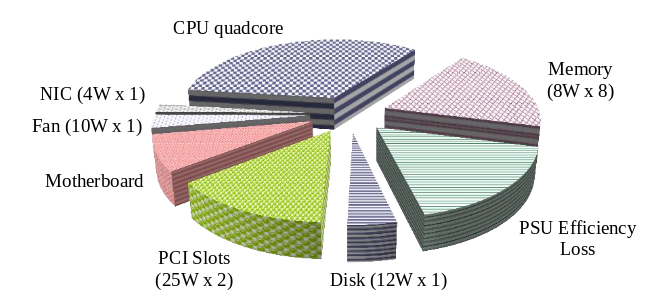
\includegraphics[scale=.4]{imagens/consumos.png}
%    \caption{Power consumption by server %components~\cite{Nathuji}}
 %   \label{fig:consumos}
%\end{figure}


%terminar
In contrast, dynamic power ranges of all the other server components are much narrower: less than 50\% for Dynamic Random Access Memory (DRAM), 25\% for disk drives, 15\% for network switches, and negligible for other components~\cite{fan2007power}. The reason is that only the CPU supports active low-power modes, whereas other components can only be completely or partially switched off. However, the performance overhead of a transition between the active and inactive modes is substantial. For example, a disk drive in the deep-sleep mode consumes almost no power, but a transition to the active mode incurs a latency 1000x  higher than the regular access latency. Power inefficiency of the server components in the idle state leads to a narrow overall dynamic power range of 30\%: even if a server is completely idle, it still consumes more than 70\% of its peak power.

The adoption of multi-core CPUs, that are substantially more efficient than conventional single-core processors, along with the increasing use of virtualization and data-intensive applications resulted in the growing amount of memory in servers. In contrast to the CPU, DRAM has a narrower dynamic power range, and power consumption by memory chips is increasing~\cite{beloglazov2013energy}.


But, even with this energy reductions and the flexibility by the virtualization, datacenters consumes 1.4\% of the whole world energy~\cite{awada2014energy}.

%\subsection{Problems of High Power and Energy Consumption}
%In 2005 the electricity use by servers worldwide – including their associated cooling and auxiliary equipment – cost 7.2 billion dollars, it was the double comparing with the consumption in 2000 \cite{koomey2007estimating}.  The number of transistors integrated into today’s Intel Itanium 2 processor reaches nearly 1 billion. If the transistor density continues to growth, the heat (per cm2) produced by future processors would exceed that of the surface of the Sun~\cite{koch2005discovering}. The scope of energy-efficient design is not limited to main computing components (e.g., processors, storage devices, and visualization facilities), but can expand into a much larger range of resources associated with computing facilities including auxiliary equipment, water used for cooling, and even the floor space occupied by the resources~\cite{beloglazov2013energy}.

\section{Case Study}\label{sec:study}
Our case of study consists in to stress CPU and memory with the benchmark Stress-NG~\cite{STRESSNG} and then compare to see how much which one affects in a machine energy consumption and when a VM can be migrated to a node or a machine shutdown to save energy.   %falar o que vai ser testado. definir NUMA

%is a method of configuring a cluster of microprocessor in a multiprocessing system so that they can share memory locally, improving performance and the ability of the system to be expanded. 
All of our tests were made in a NUMA (non-uniform memory access) architecture machine, AMD Opteron with 64 cores, 128GB of memory and Ubuntu 14.02 LTS 64 bits. Our tests consists in doing stress on CPU and memory to see what is the impact in the current power consumption. For this, in both tests we use the tool stress-ng. To get the current power consumption, we use the tool free ipmi~\cite{freeIPMI}.


\subsection{CPU test}
In our CPU test, we get the current consumption while we charge all 64 cores in: 10\%, 20\%, 30\%, 40\%, 50\%, 60\%, 70\%, 80\%, 90\% and 100\%. %The stress-ng method used for this its: stress-ng --cpu 64 --cpu-load.


Two method are chosen to make this test in CPU, the first is \textit{cpu N:} start N workers exercising the CPU by sequentially working through all the different CPU stress methods. Instead of exercising all the CPU stress methods, one can specify a specific CPU stress method with the -cpu-method option.


And the second is \textit{CPU-load P:} load CPU with P percent loading for the CPU stress workers. 0 is effectively a sleep (no load) and 100 is full loading. The loading loop is broken into compute time (load\%) and sleep time (100\% -load\%). Accuracy depends on the overall load of the processor and the responsiveness of the scheduler, so the actual load may be different from the desired load. Note that the number of bogo CPU operations may not be linearly scaled with the load as some systems employ CPU frequency scaling and so heavier loads produce an increased CPU frequency and greater CPU bogo operations.


The figure~\ref{fig:usageCPU} show the energy consumption according with the use of CPU.
\begin{figure}[]
    \centering
    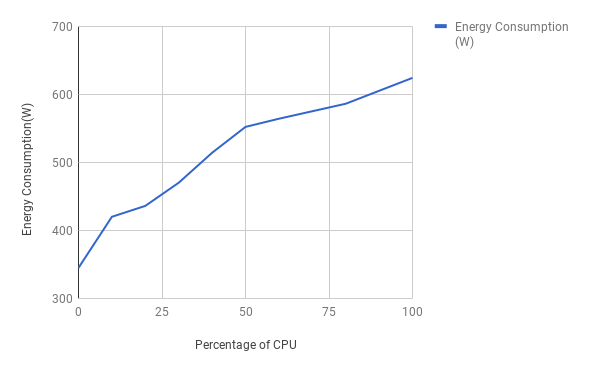
\includegraphics[scale=0.6]{imagens/CPU.png}
    \caption{Energy Consumption by CPU}
    \label{fig:usageCPU}
\end{figure}
%trocar high para underload
%trocar low para overload
%mudar razoavel para normal
%mudar limitado par underuse
%mudar elevado para overload
% stress-ng -c 64  --cpu-load 20 --timeout 40s
%graficos
%memoria:
%ate 20 >> baixo
%entre 20 e 30 é baixo e médio
%entre 30 e 80 é médio
%de 70 até o fim é alto
%prioridade deigrar vm para um nodo (utilização):
%low > entre 0 e 40
%limitado > entre 10 e 90 
%alto > de 55 ate 100
%uso CPU:
%entre 0 e 30 > limitado
%entre 20 e 80 > razoavel
%entre 70 e 100 > elevado
\subsection{Memory test}
In our Memory test, we get the current consumption while we do write and read about a certain percentage of all 128GB memory: 20\%, 40\%, 60\%, 80\% and 100\%.
%refazer abstract
%explicar como se chegou do gráfico para o fuzzy


Two method are chosen to make this test in memory, the first is \textit{memrate N:}
start  N  workers  that  exercise  a  buffer  with  64,  32,  16  and  8 bit  reads  and  writes.  This  memory stressor  allows  one  to  also  specify  the  maximum  read  and  write  rates.  The  stressors  will  run  at maximum speed if no read or write rates are specified.
And the second is \textit{memrate-bytes:} specify the size of the memory buffer being exercised. The default size is 256MB. One can specify
the size in units of Bytes, KBytes, MBytes and GBytes using the suffix b, k, m or g.
The size limit of memrate-bytes is 4GB, so, for our tests we divide the memory to reach the percentage that we need to test.

The table~\ref{tab:table} show the energy consumption by the use of memory, for that we had to use a minimun of CPU that allocate and makes writes/reads, each core can lead with 4GB of memory. (i.e, 50\% of CPU means 32 cores, that each one will manage 4GB of memory doing reads and writes, totalizing 128GB of memory). The case where CPU is on 0\% and memory does not have nothing means that the machine is idle.

% ADICIONAR DESCRIÇÃO NA TABELA @@@@@@@@@@@@@@@@@@@@@@@@@@@@@@@@@@@@@@@@@ ++ Lembrar do Idle
\begin{table}[]
\centering
\caption{Table of Memory Energy Consumption}
\label{tab:table}
\begin{tabular}{|c | c | c |}
CPU(\%) & Memory(\%) & EnergyConsumption(W) \\
0       &            & 345                  \\
10      & 20         & 444                  \\
20      & 40         & 544                  \\
30      & 60         & 642                  \\
40      & 80         & 700                  \\
50      & 100        & 780                 
\end{tabular}
\end{table}


The figure~\ref{fig:memgraphic} shows the energy consumption on table~\ref{tab:table} minus the energy consumption in figure~\ref{fig:usageCPU}, so that removing the others server components it remains only the memory energy consumption.
\begin{figure}[H]
    \centering
    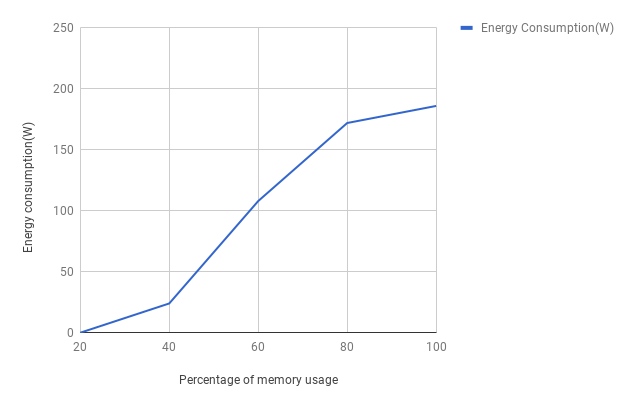
\includegraphics[scale=.6]{imagens/DRAM.png}
    \caption{Energy Consumption by Memory}
    \label{fig:memgraphic}
\end{figure}



%stress-ng --memrate-bytes $(awk '/MemFree/{printf "%d\n", $2 * 0.2;}' < /proc/meminfo)k --memrate 1 --timeout 125s

%graficos

%write and read
%acho que as imagens ficaram mto grandes mesmo ahuahau

\subsection{Results}%\label{sec:results}
%tabela
%\textbf{grafico}
%o artigo ta com uns espaçamentos meio toscos pq eu coloquei [H] pra fixar as imagens
%não tem que falar algo de quem é o especialista?psé, quems eria?kkk  nao sei, tu que gerou a parte fuzzy :p hahauah, acho que da pra tentar justificar pelo próprio consumo, sei la. foda é ter essa referencia em si
 
We generate a Fuzzy analysis about the results with two inputs and one output. The first input is the CPU usage, the functions were defined by the results of our energy consumption test, always trying to don't have performance loss~\cite{Haydar}. The other input is the Memory usage, we define these functions analysing the energy consumption percent of memory per Watt, trying to allocate VMs in machines that have a bad memory utilization considering the energy consumption and always looking for don't have performance loss. The output is the priority that the machine have to receive VMs considering the CPU and Memory usage.
%that the priority gets higher when the cost of porcent of memory per Watt

Figure~\ref{fig:CPU} show the use of CPU is adapted to a standard scale, and the linguistic terms for fuzzy systems used are: ``underuse'' ,``normal'' and ``overloaded''. Being $P = c$ and $c \in [0;10]$.
%and if is ``underutilized", ``normal" or ``overloaded" according. Until 30\% of usage, the CPU its considerable underuse, with a little of degree of membership in medium. From 20\% until 80\% the CPU usage is medium, with little degree of membership in overload and underuse. From 70\% untill 100\%, the CPU is overload, with a little degree of membership in medium.
%trocar medium to normal
\begin{figure}[H]
    \centering
    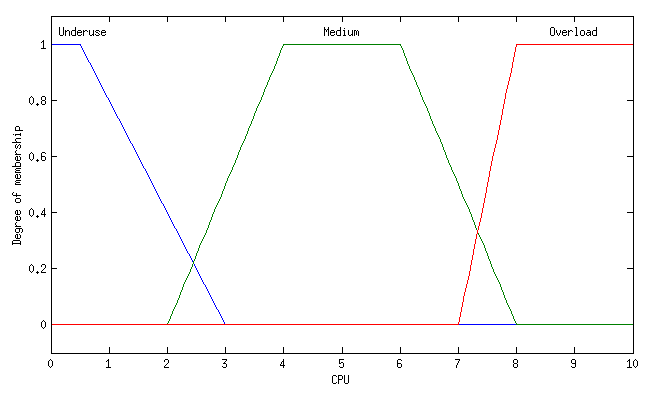
\includegraphics[scale=.7]{imagens/cpu.png}
    \caption{CPU in the default scale}
    \label{fig:CPU}
\end{figure}




The figure~\ref{fig:memoria} show the use of Memory is also adapted to a standard scale, and the linguistic terms for fuzzy systems used are: ``underuse'' ,``normal'' and ``overloaded''. Being $P = c$ and $c \in [0;10]$.
\begin{figure}[H]
    \centering
    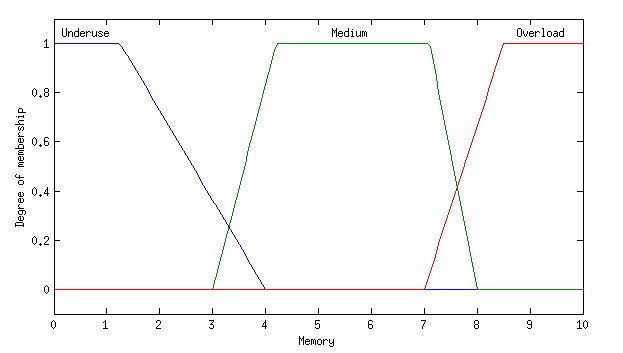
\includegraphics[scale=.7]{imagens/memoria.png}
    \caption{Memory in the default scale}
    \label{fig:memoria}
\end{figure}



For the output, the results lead us to the figure~\ref{fig:prioridade}, which show the degree of membership about a machine and if it can receive a VM in a node. This Fuzzy system is also adapted to a standard scale, and the linguistic terms for fuzzy systems used are: ``Low'' ,``normal'' and ``High''. Being $P = c$ and $c \in [0;10]$.
With this, we can classify the use of a machine based on its energy consumption,
if they need to be shutdown because it is in underuse or if they need to be scheduled to another node because they don't have resources anymore.
\begin{figure}[H]
    \centering
    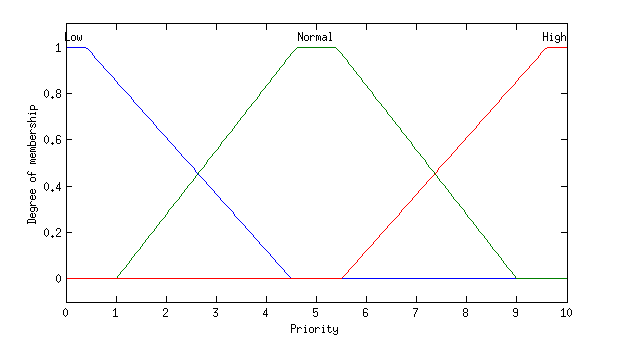
\includegraphics[scale=0.7]{imagens/prioridade.png}
    \caption{Migration Priority Membership Function}
    \label{fig:prioridade}
\end{figure}


%adicionar funções


%aqui é mostrado a prioridade de se migrar uma vm para um nodo, de 0 até 40 o grau de pertinência de se fazer uma migração é baixo, pois de acordo com as regras já vistas, não há recursos disponíveis.entre 10 e 90 é normal (verificar as pertinencias)de 50 ate 100 a prioridade é alta, o que permite a migração ou o desligamento da máquina possibilitando reduzir o consumo.

%com isso, é possivel entao classificar o uso de uma maquina tomando como ponto de partida o seu consumo energético, permitindo que seja feito o balanceamento de carga, escalonamento ou o desligamento da mesma.


In order to define the machine use, we did nine rules to help in this decision, figure~\ref{fig:regras} show they.
\begin{figure}[H]
    \centering
    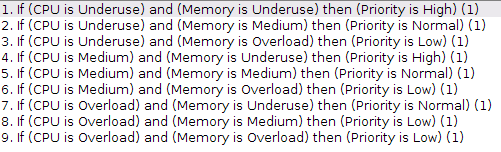
\includegraphics[scale=0.7]{imagens/regras.png}
    \caption{Fuzzy rules}
    \label{fig:regras}
\end{figure}

%lembretes:
%-- adicionar conteudo Fuzzy. check [ x ]
%-- testes [ x ]


%pegar algum do métodos do duarte para o testes
%testes:
%consumo de memória baixo e CPU baixo
%memória alta e CPU alta
%memória de 0 a 100% e CPU baixo
% memória baixo e CPU aumentando de 0 a 100%
%[ x ]

\section{Conclusion}\label{sec:conclusion}
The good management of resources in a cloud can save energy that is wasted with idle machines that could be poweroff and avoiding loss performance by scheduling machines overloaded by VMs.

To help this management, the classification of a machine by your energy consumption can save resources put machines which are underused in poweroff and do load balance in machines which are overload. Besides that, this kind of analysis also covers non-volatile memory that are considered the next step on memory technology~\cite{mittal2015survey}.

For the future works, we will propose a extension to type-2 Fuzzy Logic that treats the uncertainties associated with fuzzy sets which is not contemplated in fuzzy logic type 1.


%como trabalhos futuros, tem-se a aplicação da lógica fuzzy tipo 2 a esses dados com o intuito de abrangir o que a lógica fuzzy tipo 1 não abrangiu.

%os estudos feitos possibilitam futuramente fazer analises em memórias volateis




%\bibliographystyle{sbc}
%\bibliography{sbc-template}

\bibliographystyle{splncs} 
\bibliography{main}


\end{document}